\documentclass[tikz,border=3pt]{standalone}
\usepackage{amsmath}
\usepackage{tikz}
\begin{document}
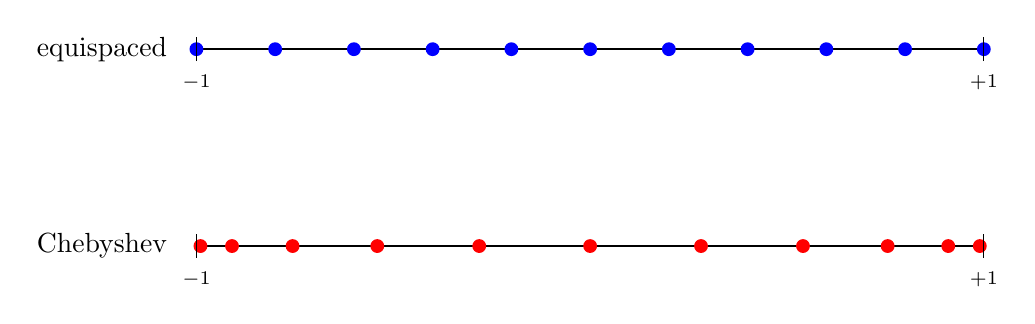
\begin{tikzpicture}[scale=5]
  % Top row: equispaced nodes on [-1,1], n=11
  \draw[thick] (-1,0.5) -- (1,0.5);
  \foreach \k in {0,1,...,10} {
    \pgfmathsetmacro{\xe}{-1 + \k*2/10}
    \fill[blue] (\xe,0.5) circle (0.5pt);
  }
  \node[left] at (-1.05,0.5) {equispaced};
  % tick marks at endpoints
  \draw (-1,0.47) -- (-1,0.53);
  \draw ( 1,0.47) -- ( 1,0.53);
  \node[below] at (-1,0.46) {\scriptsize $-1$};
  \node[below] at ( 1,0.46) {\scriptsize $+1$};

  % Bottom row: Chebyshev nodes cos((2k-1)*pi/22), k=1..11
  \draw[thick] (-1,0) -- (1,0);
  \foreach \k in {1,2,...,11} {
    \pgfmathsetmacro{\xc}{cos((2*\k-1)*180/22)}
    \fill[red] (\xc,0) circle (0.5pt);
  }
  \node[left] at (-1.05,0) {Chebyshev};
  \draw (-1,-0.03) -- (-1,0.03);
  \draw ( 1,-0.03) -- ( 1,0.03);
  \node[below] at (-1,-0.04) {\scriptsize $-1$};
  \node[below] at ( 1,-0.04) {\scriptsize $+1$};
\end{tikzpicture}
\end{document}
